\chapter{SYSTEM ARCHITECTURE AND METHODOLOGY}
\label{chap:methodology}

\section{System Overview}

The system follows an eight-stage pipeline architecture:
\begin{enumerate}
    \item Data ingestion
    \item Data preprocessing
    \item Feature engineering
    \item Feature selection
    \item Baseline model development
    \item Deep learning model training
    \item Model validation
    \item 2026 ENSO forecasting
\end{enumerate}
The framework ingests multi-variable climate reanalysis data and produces ENSO state predictions at 6-month lead times along with regional precipitation and temperature anomaly forecasts for South Asia.

\section{System Architecture}

\begin{figure}[H]
    \centering
    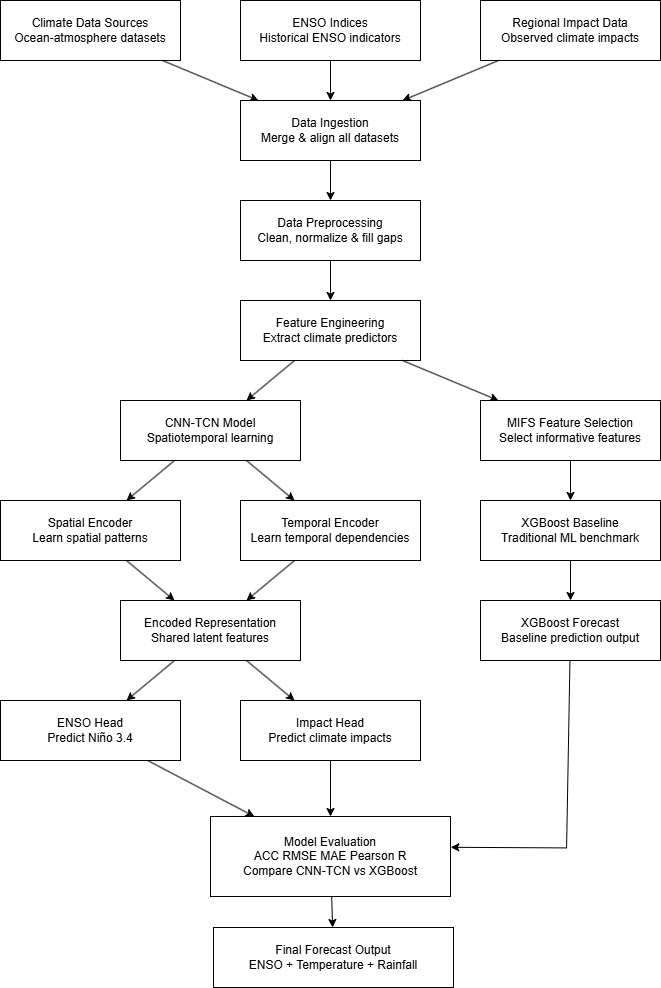
\includegraphics[width=0.85\textwidth]{src/images/system_architecture.png}
    \captionsetup{justification=centering}
    \caption{System Architecture of the project}
    \label{fig:system_architecture}
\end{figure}

The system architecture comprises eight sequential stages: (1) \textbf{Data Ingestion}, where multi-variable climate reanalysis datasets (ERA5, ORAS5, NOAA) are acquired from public repositories; (2) \textbf{Data Preprocessing}, which includes spatial standardization to a uniform 2\degree$\times$2\degree\ grid, temporal alignment to the common period 1980--2025, climatological anomaly computation, and z-score normalization; (3) \textbf{Feature Engineering}, where 12-month sliding window input tensors of shape $(12 \times 30 \times 100 \times 6)$ are constructed from the six spatial fields; (4) \textbf{Feature Selection}, applying Mutual Information Feature Selection (MIFS) for the XGBoost baseline; (5) \textbf{Baseline Model Development}, comprising the XGBoost baseline; (6) \textbf{Deep Learning Model Training}, comprising the CNN-TCN deep learning model; (7) \textbf{Model Validation}, where the models are evaluated; and (8) \textbf{Forecasting}, where the trained model generates 3-month and 6-month lead Ni\~{n}o 3.4 index predictions and regional South Asian precipitation and temperature anomaly forecasts.

\begin{figure}[H]
    \raggedleft
    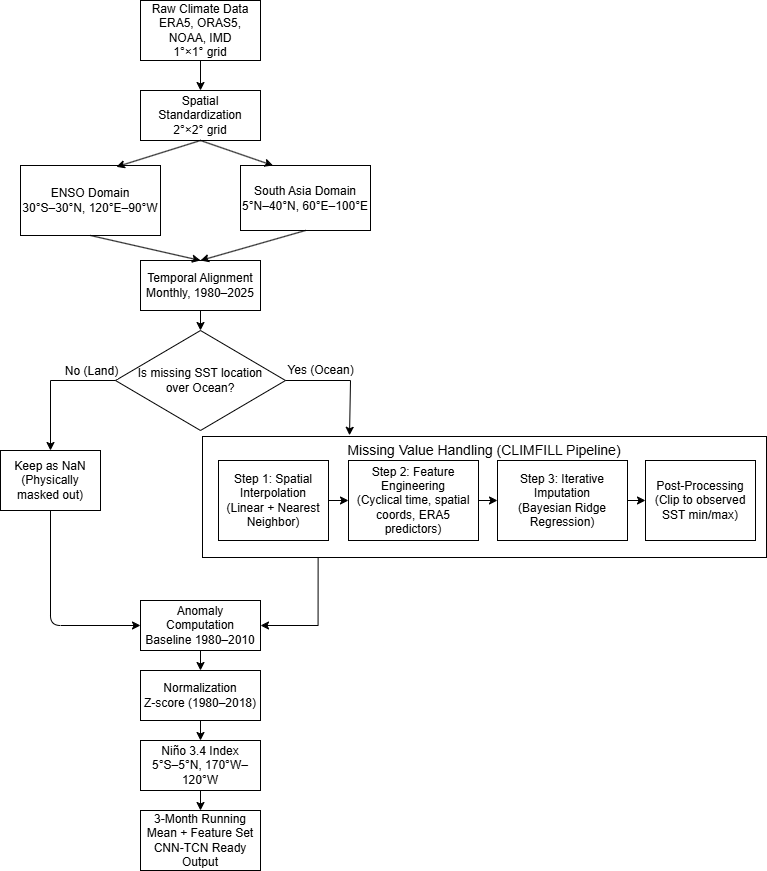
\includegraphics[width=0.85\textwidth]{src/images/data_preprocess.png}
    \captionsetup{justification=centering}
    \caption{Data Preprocessing Pipeline}
    \label{fig:data_preprocess}
\end{figure}

The data preprocessing pipeline (Figure \ref{fig:data_preprocess}) transforms raw climate reanalysis fields into analysis-ready inputs through four sequential operations: spatial standardization via area-weighted block averaging to a 2\degree$\times$2\degree\ grid, temporal alignment ensuring all variables share the 1980--2025 monthly time axis, climatological anomaly computation by subtracting the long-term monthly mean, and z-score normalization to scale all fields to have a mean of 0 and a standard deviation of 1 for stable model training.

\section{Data Sources}

The project utilizes the following publicly available datasets:

\subsection{Oceanic \& Atmospheric Reanalysis}
\begin{itemize}
    \item \textbf{ERA5 Reanalysis (ECMWF):} Monthly SST, sea level pressure (SLP), 2m temperature (T2M), and wind stress fields at 1\degree$\times$1\degree\ resolution (1950--2025).
    \item \textbf{ORAS5 (ECMWF):} Ocean heat content and subsurface temperature profiles for the tropical Pacific.
\end{itemize}

\subsection{ENSO Indices}
\begin{itemize}
    \item \textbf{Ni\~{n}o 3.4 Index (NOAA):} Monthly SST anomaly in the Ni\~{n}o 3.4 region (5\degree N--5\degree S, 170\degree W--120\degree W), serving as the primary ENSO indicator (1871--present).
\end{itemize}

\section{Workflow}

The project follows an eight-step pipeline: data ingestion, data preprocessing, feature engineering, feature selection, baseline model development, deep learning model training, model validation, and 2026 forecasting. The data-facing steps of this pipeline are described below; the feature selection strategy, the baseline model, and the deep learning model are each developed in dedicated sections (Sections~\ref{sec:feature-selection}--\ref{sec:cnn-tcn}) given the depth of methodological detail each requires.

\subsection{Data Ingestion}
All datasets are aggregated, resampled to a consistent monthly 2\degree$\times$2\degree\ grid, and aligned to the common period 1980--2025. Data quality checks and gap-filling procedures are applied to ensure temporal continuity.

\subsection{Data Preprocessing}

The raw climate datasets ingested from ERA5, ORAS5, and NOAA undergo the following preprocessing steps prior to feature engineering:

\noindent\textbullet\ \textbf{Spatial Standardization}\\
All datasets are ingested at their native 1\degree\ latitude $\times$ 1\degree\ longitude spatial resolution. A 1\degree\ latitude $\times$ 1\degree\ longitude grid cell covers approximately 111 km (along latitude) $\times$ 111 km (along longitude) at the equator, representing an area of roughly 12,300 km\textsuperscript{2}. At 27\degree N (Nepal/India region), 1\degree\ longitude shrinks to approximately 99 km, making each 1\degree\ latitude $\times$ 1\degree\ longitude cell approximately 111 km $\times$ 99 km $\approx$ 10,989 km\textsuperscript{2}. All datasets are subsequently coarsened to a 2\degree\ latitude $\times$ 2\degree\ longitude grid using block averaging (area-weighted mean over each 2 $\times$ 2 grid cell block), where each coarsened cell covers approximately 222 km $\times$ 198 km $\approx$ 43,956 km\textsuperscript{2} at 27\degree N, roughly 30\% of Nepal's total land area. This spatial coarsening reduces the total data volume by a factor of four while preserving the large-scale spatial patterns and teleconnection signals critical for ENSO dynamics, as the dominant modes of interannual Sea Surface Temperature (SST) variability operate at spatial scales well above the 2\degree\ threshold. The coarsened fields are then clipped to the tropical Pacific (30\degree S--30\degree N, 120\degree E--80\degree W) for ENSO modeling and to South Asia (5\degree N--40\degree N, 60\degree E--100\degree E) for regional impact assessment.

\noindent\textbullet\ \textbf{Temporal Alignment}\\
All variables are resampled to a consistent monthly temporal resolution and aligned to the common period 1980--2025, yielding 552 monthly time steps. ERA5 fields are aggregated as monthly means, and missing time steps are identified and flagged for gap-filling.

\noindent\textbullet\ \textbf{Missing Value Handling (CLIMFILL Pipeline)}\\
Missing values in the Sea Surface Temperature (SST) variable, arising from datatype inconsistencies and land-sea boundaries, are handled using a three-step CLIMFILL-style pipeline. Crucially, this pipeline is applied strictly to ocean points (identified via the land-sea mask, \texttt{lsm} $<$ 0.5), while land points are intentionally left as \texttt{NaN} to prevent physical contamination of the dataset.

\textbf{Step 1: Spatial Interpolation (First-Guess):} A spatial first-guess is generated for every oceanic gap by interpolating SST across latitude and longitude within each monthly time slice. Using the \texttt{griddata} function from the \texttt{scipy.\allowbreak interpolate} module, linear interpolation estimates missing values from surrounding valid ocean points. For gaps falling outside the convex hull of known data, a nearest-neighbor fallback method is applied.

\textbf{Step 2: Multivariate Feature Engineering:} To refine the spatial estimates, a robust set of multivariate predictors is engineered. Temporal seasonality is captured via cyclical sine and cosine transformations of the month. Spatial context is retained using latitude, longitude, and the spatial first-guess. Furthermore, highly correlated atmospheric variables from ERA5, including 2-meter temperature, mean sea level pressure, wind components, and top-of-atmosphere thermal radiation, are incorporated to inform the imputation.

\textbf{Step 3: Iterative Multivariate Imputation:} The final step employs an iterative algorithm to refine the SST estimates. Using the \texttt{Iterative\allowbreak Imputer} from the \texttt{scikit-learn} library with a \texttt{Bayesian\allowbreak Ridge} regression estimator, the model iteratively predicts missing values based on the engineered features. This runs for a maximum of 10 iterations until convergence, strictly preserving all originally observed SST values.

\textbf{Post-Processing:} To ensure physical realism, the refined SST estimates are clipped to the minimum and maximum bounds of the originally observed oceanic SST range. This prevents the statistical model from generating extreme outliers and ensures the imputed data remains physically plausible.

\textbf{Variable Exclusion:} Variables for which more than 5\% of total data points, computed across all time steps and grid cells, remain missing after the application of the above filling strategies are excluded entirely from the feature set. Retention of heavily incomplete variables risks introducing spurious patterns into the training data, potentially degrading model performance.

\noindent\textbullet\ \textbf{Anomaly Computation}\\
\label{sec:anomaly}
Monthly climatological means are computed for each variable over the 1980--2010 baseline period and subtracted from the raw fields to obtain anomaly fields. This removes the seasonal cycle and isolates interannual variability relevant to ENSO dynamics:
\begin{equation}
    X'(t) = X(t) - \bar{X}_{m}
\end{equation}
where $X'(t)$ is the anomaly at time $t$, $X(t)$ is the raw value, and $\bar{X}_{m}$ is the climatological mean for calendar month $m$.

\noindent\textbullet\ \textbf{Normalization}\\
All anomaly fields are standardized using Z-score normalization computed exclusively on the training set (1980--2018) to prevent data leakage into the validation and test sets:
\begin{equation}
    \hat{X}(t) = \frac{X'(t) - \mu_{\text{train}}}{\sigma_{\text{train}}}
\end{equation}
where $\mu_{\text{train}}$ and $\sigma_{\text{train}}$ are the mean and standard deviation of the training period anomalies.

\noindent\textbullet\ \textbf{Ni\~{n}o 3.4 Index Computation}\\
The target variable for the El Ni\~{n}o--Southern Oscillation (ENSO) forecasting objective is the Ni\~{n}o 3.4 index, defined as the area-averaged Sea Surface Temperature (SST) anomaly over the Ni\~{n}o 3.4 region (5\degree S--5\degree N, 170\degree W--120\degree W). The index is computed directly from ERA5 SST anomaly fields, which are already ingested as part of the primary dataset pipeline, thereby eliminating the need for an additional observational dataset.

For each monthly time step $t$, the Ni\~{n}o 3.4 index is computed as the area-weighted spatial mean of SST anomalies over all grid cells $(i,j)$ falling within the Ni\~{n}o 3.4 domain:

\begin{equation}
    N_{3.4}(t) = \frac{\sum_{i,j \in \Omega} w(i,j) \cdot X'_{\text{SST}}(i,j,t)}{\sum_{i,j \in \Omega} w(i,j)}
\end{equation}

\noindent where $N_{3.4}(t)$ is the Ni\~{n}o 3.4 index at time step $t$, $X'_{\text{SST}}(i,j,t)$ is the SST anomaly at grid cell $(i,j)$ and time step $t$ computed following the anomaly procedure described in Section~\ref{sec:anomaly}, $\Omega$ denotes the set of all grid cells within the Ni\~{n}o 3.4 region (5\degree S--5\degree N, 170\degree W--120\degree W), and $w(i,j) = \cos(\phi_i)$ is the area weight assigned to grid cell $(i,j)$, where $\phi_i$ denotes the latitude of grid cell $i$ in radians.

A 3-month running mean is subsequently applied to the raw monthly index values to suppress intra-seasonal noise and retain only the multi-month ENSO signal:

\begin{equation}
    \hat{N}_{3.4}(t) = \frac{1}{3} \sum_{k=0}^{2} N_{3.4}(t-k)
\end{equation}

\noindent where $\hat{N}_{3.4}(t)$ is the smoothed Ni\~{n}o 3.4 index at time step $t$ and $N_{3.4}(t-k)$ denotes the raw index value at lag $k$ months. The resulting smoothed time series serves as the primary prediction target for the CNN-TCN model in Objective 1 and as the conditioning variable for the regional impact assessment module in Objective 2.

\subsection{Feature Engineering}
\label{sec:feature-engineering}
Input sequences are constructed consisting of 12 consecutive monthly snapshots of six spatial fields extracted over the tropical Pacific domain (30\degree S--30\degree N, 120\degree E--80\degree W), which represents the primary region of El Ni\~{n}o--Southern Oscillation (ENSO) variability. The six spatial fields are as follows:

\begin{itemize}
    \item \textbf{Sea Surface Temperature (SST) anomaly}, sourced from the European Centre for Medium-Range Weather Forecasts Reanalysis version 5 (ERA5), representing the primary indicator of ENSO state at the ocean surface.
    \item \textbf{Mean Sea Level Pressure (MSL) anomaly}, sourced from ERA5, capturing the atmospheric pressure patterns associated with the Walker Circulation and trade wind variability.
    \item \textbf{Zonal (east--west) wind stress anomaly}, sourced from ERA5, representing the strength and direction of trade winds along the equatorial Pacific, which drive the east-west redistribution of warm surface water characteristic of ENSO events.
    \item \textbf{Meridional (north--south) wind stress anomaly}, sourced from ERA5, capturing cross-equatorial wind dynamics and their role in ENSO evolution.
    \item \textbf{Upper 300m Ocean Heat Content (OHC) anomaly}, sourced from the Ocean Reanalysis System 5 (ORAS5), capturing subsurface thermal energy accumulation in the tropical Pacific. Subsurface heat content is among the most skillful predictors of ENSO at lead times of 3 months and beyond, as it reflects the recharge and discharge of oceanic heat prior to the surface expression of El Ni\~{n}o or La Ni\~{n}a events.
    \item \textbf{20\degree C Isotherm Depth anomaly}, sourced from ORAS5, representing thermocline depth variations in the equatorial Pacific, which serve as a critical physical precursor to surface SST changes.
\end{itemize}

Each input sequence is therefore represented as a four-dimensional tensor of shape:

\begin{equation}
\mathbf{X} \in \mathbb{R}^{T \times N_{\phi} \times N_{\lambda} \times C}
\end{equation}

\noindent where $T = 12$ denotes the number of monthly time steps in each input window, $N_{\phi} = 30$ denotes the number of latitude grid cells, $N_{\lambda} = 100$ denotes the number of longitude grid cells, and $C = 6$ denotes the number of input channels corresponding to the six spatial fields listed above. These sequences serve as the primary input to both the Convolutional Neural Network--Temporal Convolutional Network (CNN-TCN) model and the XGBoost baseline model, with the latter receiving the tensor flattened into a one-dimensional feature vector of length $12 \times 30 \times 100 \times 6 = 216{,}000$ prior to MIFS-based dimensionality reduction (Section~\ref{sec:feature-selection}).



\subsection{Validation and Evaluation}
A chronological train--validate--test split is employed to evaluate model performance, ensuring that no future information is accessible during training or validation:

\begin{itemize}
    \item \textbf{Training:} 1980--2018
    \item \textbf{Validation:} 2019--2022
    \item \textbf{Testing:} 2023--2025
\end{itemize}

\noindent Hyperparameters for both the Convolutional Neural Network--Temporal Convolutional Network (CNN-TCN) and the XGBoost baseline are tuned exclusively on the validation set. Final performance for both models is reported on the held-out test set (2023--2025).

\textbf{ENSO Forecast Evaluation:} The performance of the Ni\~{n}o 3.4 index forecast is evaluated using the following metrics:

\textbf{Anomaly Correlation Coefficient (ACC):}
The ACC measures the temporal correlation between predicted and observed Ni\~{n}o 3.4 anomalies over the test period:

\begin{equation}
\text{ACC} = \frac{\sum_{t=1}^{N} \hat{y}(t) \cdot y(t)}{\sqrt{\sum_{t=1}^{N} \hat{y}(t)^{2}} \cdot \sqrt{\sum_{t=1}^{N} y(t)^{2}}}
\end{equation}

\noindent where $\hat{y}(t)$ is the predicted Ni\~{n}o 3.4 index at time step $t$, $y(t)$ is the corresponding observed value, and $N$ is the total number of test time steps. An ACC value of 1.0 indicates perfect prediction skill, while a value of 0.0 indicates no skill. A model is generally considered skillful when ACC $> 0.5$.

\textbf{Root Mean Square Error (RMSE):}
The RMSE quantifies the average magnitude of prediction errors in the same units as the Ni\~{n}o 3.4 index (\degree C):

\begin{equation}
\text{RMSE} = \sqrt{\frac{1}{N} \sum_{t=1}^{N} \left( \hat{y}(t) - y(t) \right)^{2}}
\end{equation}

\noindent where a lower RMSE indicates better forecast accuracy. Both ACC and RMSE are reported for the CNN-TCN and XGBoost models to enable direct comparison.

\textbf{Impact Forecast Evaluation:} The performance of the South Asia precipitation and temperature anomaly forecasts is evaluated against ERA5 reanalysis data using the following metrics:

\textbf{Mean Absolute Error (MAE):}
The MAE measures the average absolute deviation between predicted and observed anomaly values across all South Asian grid cells and test time steps:

\begin{equation}
\text{MAE} = \frac{1}{N \cdot G} \sum_{t=1}^{N} \sum_{g=1}^{G} \left| \hat{y}(g,t) - y(g,t) \right|
\end{equation}

\noindent where $\hat{y}(g,t)$ is the predicted anomaly at grid cell $g$ and time step $t$, $y(g,t)$ is the corresponding observed anomaly, $G = 340$ is the total number of South Asian grid cells, and $N$ is the number of test time steps.

\textbf{Pearson Correlation Coefficient:}
The Pearson correlation coefficient measures the linear association between predicted and observed anomaly fields across all grid cells and test time steps:

\begin{equation}
r = \frac{\sum_{t=1}^{N} \sum_{g=1}^{G} \left( \hat{y}(g,t) - \bar{\hat{y}} \right) \left( y(g,t) - \bar{y} \right)}{\sqrt{\sum_{t=1}^{N} \sum_{g=1}^{G} \left( \hat{y}(g,t) - \bar{\hat{y}} \right)^{2}} \cdot \sqrt{\sum_{t=1}^{N} \sum_{g=1}^{G} \left( y(g,t) - \bar{y} \right)^{2}}}
\end{equation}

\noindent where $\bar{\hat{y}}$ and $\bar{y}$ are the mean predicted and observed anomaly values respectively across all grid cells and test time steps. A Pearson correlation value closer to 1.0 indicates stronger agreement between the predicted and observed spatial anomaly patterns.

\subsection{2026 Forecasting}
Generate ensemble forecasts for the Ni\~{n}o 3.4 index and June--July--August--September 2026 precipitation and temperature anomalies over South Asia using the trained model with the most recent available observational data as input.

\section{Feature Selection}
\label{sec:feature-selection}

\subsection{Overview of the Feature Selection Strategy}
\label{sec:fs-overview}

The XGBoost baseline receives the fully flattened input tensor as a tabular feature vector of $12 \times 30 \times 100 \times 6 = 216{,}000$ dimensions per sample (Section~\ref{sec:feature-engineering}), while only on the order of a few hundred labelled monthly samples are available across the 1980--2025 study period. Training a tree-based model directly on a feature space of this dimensionality relative to the available sample size invites severe overfitting and prohibitively slow training, motivating an explicit feature selection stage prior to baseline model development. The Convolutional Neural Network--Temporal Convolutional Network (CNN-TCN), by contrast, learns spatial feature weighting implicitly through its convolutional filters during end-to-end training and therefore requires no separate feature selection step; the discussion in this section applies exclusively to the XGBoost baseline pipeline.

Mutual Information Feature Selection (MIFS) is adopted as the feature selection criterion in preference to simpler alternatives such as univariate correlation filtering or Principal Component Analysis (PCA). Unlike Pearson correlation, mutual information captures non-linear statistical dependence between a candidate grid cell and the continuous Ni\~{n}o 3.4 target without requiring the target to be discretized into categorical ENSO phases, preserving the full information content of the regression target. Unlike PCA, MIFS retains individual, physically interpretable grid cells rather than opaque linear combinations of the input space, and its redundancy-penalized formulation directly targets the specific failure mode of concern in a spatially gridded climate field: neighbouring grid cells are typically highly autocorrelated, so a purely relevance-ranked feature set would be dominated by clusters of near-duplicate cells centered on the strongest predictor region rather than a spatially diverse set of predictors.

Computing the redundancy term of the MIFS objective (Section~\ref{sec:mifs-general}) requires the pairwise mutual information between every pair of candidate features already in, or being considered for, the selected set. Estimating this quantity accurately, via a k-nearest-neighbour (Kraskov) estimator, scales poorly with the number of candidate features under consideration, making it computationally infeasible to run an exact MIFS search directly over the full 144,000-dimensional candidate space. This creates a direct trade-off between the size of the candidate pool that can be searched and the exactness of the redundancy estimate applied to it: restricting the candidate pool keeps the exact k-NN estimator tractable but risks discarding relevant features during the initial pre-filtering step, whereas searching a substantially larger candidate pool requires replacing the exact estimator with a cheaper approximation.

Rather than committing to one side of this trade-off, two independent, complementary MIFS implementations were designed, implemented, and evaluated against each other:

\begin{itemize}
    \item \textbf{Method 1} (Section~\ref{sec:mifs-method1}) prioritizes estimator exactness. It restricts the candidate pool to a small, stratified subset of features before applying the exact k-NN-based redundancy estimator, keeping the pairwise mutual information computation tractable at the cost of a narrower search space.
    \item \textbf{Method 2} (Section~\ref{sec:mifs-method2}) prioritizes search breadth. It expands the candidate pool by an order of magnitude relative to Method 1 and substitutes a closed-form Gaussian correlation approximation for the exact redundancy estimate, trading estimator precision for the ability to search a substantially larger portion of the feature space.
\end{itemize}

Both methods share the same underlying relevance criterion, redundancy-penalized objective, and greedy selection procedure, described generally in Section~\ref{sec:mifs-general}; they differ solely in how the candidate pool is constructed and how the pairwise redundancy term is estimated. Running both implementations to completion allows the two competing computational strategies: exact estimation over a narrow pool versus approximate estimation over a broad pool: to be compared directly on held-out validation performance, with the corresponding experimental results reported in Chapter~\ref{chap:implementation}.

\subsection{Mutual Information Feature Selection}
\label{sec:mifs-general}

\textbf{Mutual Information:} For each grid cell $(i,j)$ of each input variable, the mutual information between the grid cell values and the continuous Ni\~{n}o 3.4 target is computed as:

\begin{equation}
I(X_{i,j}; Y) = \sum_{x \in X_{i,j}} \sum_{y \in Y} p(x, y) \log \frac{p(x, y)}{p(x)\, p(y)}
\end{equation}

\noindent where $X_{i,j}$ denotes the values of the feature at grid cell $(i,j)$ across all training samples, $Y$ denotes the corresponding continuous Ni\~{n}o 3.4 index values, $p(x,y)$ is the joint probability distribution of $X_{i,j}$ and $Y$, and $p(x)$ and $p(y)$ are the respective marginal probability distributions. A high value of $I(X_{i,j}; Y)$ indicates that knowing the value at grid cell $(i,j)$ substantially reduces uncertainty about the Ni\~{n}o 3.4 index, implying strong predictive relevance for ENSO forecasting.

\textbf{Redundancy Penalization:} MIFS explicitly penalizes redundancy between candidate and already selected features to ensure the retained feature set is both maximally informative and minimally redundant. For a candidate feature $X_{i,j}$ and the set of already selected features $S$, the redundancy-penalized relevance score is defined as:

\begin{equation}
S(X_{i,j}) = I(X_{i,j}; Y) - \frac{1}{|S|} \sum_{X_{k,l} \in S} I(X_{i,j}; X_{k,l})
\end{equation}

\noindent where $I(X_{i,j}; Y)$ is the mutual information between the candidate feature and the Ni\~{n}o 3.4 target, $I(X_{i,j}; X_{k,l})$ is the mutual information between the candidate feature and each already selected feature $X_{k,l} \in S$, and $|S|$ is the current size of the selected feature set. At each iteration, the candidate feature with the highest score $S(X_{i,j})$ is added to $S$. This iterative procedure ensures that each newly selected feature contributes maximum new predictive information about the Ni\~{n}o 3.4 target beyond what the already selected features collectively provide.

\textbf{General Algorithm:} Given a candidate pool of features, the greedy MIFS procedure proceeds as follows:

\begin{enumerate}
    \item \textbf{Compute relevance:} Calculate the mutual information relevance $I(X_{i,j}; Y)$ for every candidate feature against the Ni\~{n}o 3.4 target.
    \item \textbf{Initialize the selected set:} Set $S = \emptyset$ and, at the first iteration, select the candidate with maximum relevance alone.
    \item \textbf{Greedy redundancy-penalized selection:} At each subsequent iteration, compute the redundancy-penalized score $S(X_{i,j})$ for every remaining candidate against the current selected set and add the highest-scoring candidate to $S$.
    \item \textbf{Repeat:} Continue steps 2--3 until a predetermined number of features $K$ has been selected, yielding a ranked list of features in order of selection.
    \item \textbf{Select $K$ via K-sweep:} Since $K$ is not fixed a priori, retrain XGBoost on the top-$K$ features for a range of candidate $K$ values and evaluate each on the validation set (2019--2022), retaining the value of $K$ that minimizes validation Root Mean Square Error (RMSE) as $K^*$.
\end{enumerate}

\textbf{Physical Interpretation:} The spatial regions expected to achieve the highest mutual information scores with the Ni\~{n}o 3.4 target are consistent with established ENSO physics. Sea Surface Temperature (SST) anomalies in the central and eastern equatorial Pacific, equatorial wind stress anomalies along the Walker Circulation pathway, and upper 300m Ocean Heat Content (OHC) anomalies in the western Pacific thermocline are expected to carry the strongest predictive signal. The redundancy penalization step further ensures that highly correlated neighboring grid cells, which carry largely overlapping information, do not dominate the selected feature set, yielding a spatially diverse and physically meaningful set of predictors.

\textbf{Application:} The MIFS procedure, in both of its implementations described below, is applied exclusively to the XGBoost baseline model. The selected $K$ features are extracted from the flattened one-dimensional input vector and fed directly into XGBoost for training and inference. The CNN-TCN model receives the full unfiltered input tensor of shape $(12 \times 30 \times 100 \times 6)$ without any prior feature selection, as the spatial encoder handles all feature extraction implicitly through learned convolutional filters.

\subsection{Method 1: Stratified/Flat MIFS with Restricted Candidate Pool}
\label{sec:mifs-method1}

Method 1 applies the general MIFS procedure of Section~\ref{sec:mifs-general} while aggressively restricting the candidate pool prior to running the greedy loop, keeping the exact k-nearest-neighbour redundancy estimator computationally tractable. Candidate restriction is performed using one of two pre-filtering strategies: a flat top-$N$ cut on relevance, or a stratified, per-variable-type quota.

\textbf{Relevance Estimation:} Mutual information relevance $I(X_{i,j}; Y)$ is computed for every feature in the full 144,000-dimensional feature set using a Kraskov k-nearest-neighbour estimator, implemented via \texttt{scikit-learn}'s \texttt{mutual\_info\_regression} function with $k = 5$ neighbors, evaluated exclusively on the training partition of the chronological data split described in Chapter~\ref{chap:implementation}.

\textbf{Stratified Pre-filtering:} Rather than retaining a flat top-$N$ set of the most relevant features overall -- which risks being dominated entirely by Sea Surface Temperature (SST) grid cells, the single strongest individual predictor -- Method 1's stratified variant groups candidate features by variable type (e.g., SST, Ocean Heat Content) and applies a per-type quota:

\begin{equation}
q_{\text{type}} = \min\big(\text{cap}_{\max},\ \max(\text{cap}_{\min},\ \text{fraction} \times n_{\text{type}})\big)
\end{equation}

\noindent where $n_{\text{type}}$ is the number of candidate features belonging to a given variable type, and $\text{fraction} = 0.4$, $\text{cap}_{\min} = 15$, and $\text{cap}_{\max} = 30$ are tunable quota parameters. This stratification ensures that mechanistically important but individually weaker predictors, such as Ocean Heat Content and wind stress, are guaranteed representation in the candidate pool rather than being crowded out by SST. Applying either pre-filtering strategy yields a restricted candidate pool of at most 300 features.

\textbf{Greedy Selection and K-Sweep:} The general greedy MIFS loop of Section~\ref{sec:mifs-general} is then executed over this restricted candidate pool, with pairwise mutual information values cached to avoid redundant computation across iterations. The resulting ranked feature list is evaluated via a K-sweep over $K = 1, 2, \ldots, 50$ in steps of 2, with an XGBoost model trained on each top-$K$ subset and validated against held-out validation-period RMSE to select $K^*$. The corresponding K-sweep results are reported in Chapter~\ref{chap:implementation}.

\subsection{Method 2: Correlation-Approximated MIFS with Expanded Candidate Pool}
\label{sec:mifs-method2}

Where Method 1 trades search breadth for estimator exactness, Method 2 applies the same general MIFS procedure (Section~\ref{sec:mifs-general}) with the opposite emphasis: it searches a substantially larger candidate pool, at the cost of replacing the exact redundancy estimator with a computationally cheaper approximation. Method 2 operates on the same tensor-construction pipeline described in Section~\ref{sec:tensor-construction}, with all feature standardization and MIFS scoring fit exclusively on the training partition of the chronological data split, consistent with Method 1.

\textbf{Expanded Relevance Screening:} As in Method 1, mutual information relevance $I(X_{i,j}; Y)$ is computed between every candidate feature in the full feature set and the Ni\~{n}o 3.4 target using the same k-nearest-neighbour estimator. However, rather than collapsing this ranking into a candidate pool of at most 300 features via a flat or stratified quota, the top \textbf{3,000} features by relevance are retained as the candidate pool for the greedy loop -- an order of magnitude larger than the pool used in Method 1.

\textbf{Redundancy Approximation via Gaussian Relation:} Computing exact pairwise mutual information across a 3,000-feature candidate pool using the same k-nearest-neighbour (Kraskov) estimator applied in Method 1 is computationally intractable, as the number of pairwise evaluations required grows quadratically with candidate pool size. To make the expanded search feasible, Method 2 instead approximates pairwise mutual information analytically using the closed-form Gaussian relation:

\begin{equation}
I(X_i; X_j) \approx -\frac{1}{2}\ln\left(1 - \rho_{ij}^2\right)
\end{equation}

\noindent where $\rho_{ij}$ is the Pearson correlation coefficient between feature $X_i$ and feature $X_j$. This substitutes a single, efficiently computable matrix of pairwise correlations for the expensive k-nearest-neighbour redundancy estimate used in Method 1, at the cost of assuming approximately linear-Gaussian dependence between feature pairs -- an assumption that may not hold exactly for all pairs of spatially and physically related climate variables, but that permits redundancy to be estimated across a candidate pool an order of magnitude larger than would otherwise be tractable.

\textbf{Greedy Selection and K-Sweep:} Using the same redundancy-penalized scoring rule as Method 1 (Section~\ref{sec:mifs-general}),

\begin{equation}
S_{\text{score}}(X_{\text{cand}}) = I(X_{\text{cand}}; Y) - \frac{1}{|S|} \sum_{X_k \in S} I(X_{\text{cand}}; X_k),
\end{equation}

\noindent features are greedily added to the selected subset $S$ from the 3,000-feature candidate pool, with the redundancy term evaluated via the Gaussian approximation above. An XGBoost model is then incrementally retrained on nested top-$K$ subsets for $K \in \{10, 25, \ldots, 800\}$, with validation RMSE recorded at each step to select $K^*$. Because the candidate pool itself is an order of magnitude larger than Method 1's, the range of $K$ values swept is correspondingly wider, allowing the K-sweep to explore whether a substantially larger final feature set, drawn from a broader candidate pool, improves validation performance relative to Method 1's more tightly restricted search. The corresponding K-sweep results, selected feature counts, and a physical plausibility check of the selected grid cells are reported in Chapter~\ref{chap:implementation}.

\section{Baseline Model (XGBoost)}
\label{sec:baseline-model}

An eXtreme Gradient Boosting (XGBoost) regression model is employed as the baseline to establish a performance floor against which the developed CNN-TCN is evaluated. XGBoost operates on tabular input and therefore receives the MIFS-selected features as a flattened one-dimensional feature vector per sample, discarding the spatial and temporal structure preserved in the CNN-TCN input tensor.

The model is trained on the training period (1980--2018) to predict the Ni\~{n}o 3.4 index at a 6-month lead time. Hyperparameters including the number of estimators, maximum tree depth, and learning rate are tuned on the validation set (2019--2022) using grid search. Final performance is reported on the held-out test set (2023--2025) using the Anomaly Correlation Coefficient (ACC) and Root Mean Square Error (RMSE) as evaluation metrics, consistent with those applied to the CNN-TCN model.

\begin{itemize}
    \item \textbf{Established Benchmark:} XGBoost has been employed in prior ENSO and climate impact studies. It therefore serves as a credible and meaningful point of comparison.
    \item \textbf{Contrast with Spatiotemporal Learning:} XGBoost operates on flattened tabular input and cannot exploit the spatial structure of climate fields or the temporal evolution of monthly snapshots. This contrast directly demonstrates the value of the CNN-TCN architecture.
    \item \textbf{Standard Practice:} In deep learning research, it is expected to benchmark proposed models against a strong classical machine learning baseline. XGBoost is widely accepted as the standard choice for this role in recent ML literature.
    \item \textbf{Computational Efficiency:} XGBoost trains rapidly on CPU resources, serving as a quick sanity check that the data pipeline and preprocessing steps are functioning correctly before committing GPU resources to CNN-TCN training.
\end{itemize}

\section{Deep Learning Model (CNN-TCN)}
\label{sec:cnn-tcn}

The primary forecasting model is a multi-task hybrid Convolutional Neural Network--Temporal Convolutional Network (CNN-TCN) that simultaneously addresses both project objectives through a shared spatiotemporal encoder and two task-specific prediction heads. The hybrid architecture is motivated by the dual nature of El Ni\~{n}o--Southern Oscillation (ENSO) variability; ENSO manifests as both a spatial pattern (east-west Sea Surface Temperature (SST) gradient across the tropical Pacific) and a temporal evolution (progressive warming or cooling over multiple months), requiring dedicated components to capture each dimension independently before modeling their joint evolution.

\textbf{Stage 1: Spatial Encoder (CNN):}
A two-dimensional Convolutional Neural Network (CNN) is applied independently to each monthly snapshot within the 12-month input window. For each time step $t$, the CNN receives a spatial map of shape $(N_{\phi} \times N_{\lambda} \times C)$ where $N_{\phi} = 30$ denotes the number of latitude grid cells, $N_{\lambda} = 100$ denotes the number of longitude grid cells, and $C = 6$ denotes the number of input channels (SST anomaly, Mean Sea Level Pressure (MSL) anomaly, zonal and meridional wind stress anomalies, upper 300m Ocean Heat Content (OHC) anomaly, and 20\degree C Isotherm Depth anomaly). The CNN applies learned convolutional filters across the spatial dimensions to extract physically meaningful spatial features.

The output of the spatial encoder for each time step $t$ is a compact spatial feature vector $\mathbf{f}(t) \in \mathbb{R}^{d}$, where $d$ denotes the number of learned spatial features. Applying the CNN independently and identically across all 12 time steps yields a sequence of spatial feature vectors:

\begin{equation}
\mathbf{F} = \left[ \mathbf{f}(1), \mathbf{f}(2), \ldots, \mathbf{f}(12) \right] \in \mathbb{R}^{12 \times d}
\end{equation}

\noindent where each vector $\mathbf{f}(t)$ summarizes the spatial state of the tropical Pacific at month $t$.

\textbf{Stage 2: Temporal Encoder (TCN):}
The sequence of spatial feature vectors $\mathbf{F}$ is passed into a Temporal Convolutional Network (TCN) consisting of stacked dilated causal convolutional layers that model the temporal evolution of the extracted spatial patterns across the 12-month input window. Causal convolutions ensure that the representation at any time step is conditioned only on past and present observations, preventing information leakage from future time steps. Dilation is applied with exponentially increasing rates across successive layers:

\begin{equation}
d_l = 2^{l-1}, \quad l = 1, 2, 3, \ldots, L
\end{equation}

\noindent where $d_l$ is the dilation rate at layer $l$ and $L$ is the total number of dilated convolutional layers. This exponential dilation allows the receptive field of the network to grow exponentially with depth, enabling the temporal encoder to capture both short-range monthly patterns (1--2 months) and long-range multi-month dependencies (8--12 months) within the input window. The TCN component captures temporal evolution patterns such as:

\begin{itemize}
    \item Progressive eastward migration of the warm water pool over consecutive months.
    \item Gradual weakening or strengthening of trade winds across the 12-month window.
    \item Subsurface heat content buildup preceding the surface expression of El Ni\~{n}o or La Ni\~{n}a events.
\end{itemize}

The output of the temporal encoder is a single compact encoded representation vector $\mathbf{z} \in \mathbb{R}^{h}$ summarizing all spatiotemporal patterns extracted from the 12-month input sequence, where $h$ denotes the hidden dimension of the temporal encoder.

\textbf{Stage 3: Task-Specific Prediction Heads:} The encoded representation $\mathbf{z}$ is passed simultaneously into two independent fully connected prediction heads:

\textbf{ENSO Predictor Head (Objective 1):} A series of fully connected layers regresses the Ni\~{n}o 3.4 index at a 6-month lead time, producing a single deterministic scalar output:

\begin{equation}
\hat{y}_{\text{ENSO}} = f_{\text{ENSO}}(\mathbf{z}) \in \mathbb{R}
\end{equation}

\textbf{South Asia Impact Head (Objective 2):} A separate series of fully connected layers produces deterministic forecasts of June--July--August--September (JJAS) precipitation and temperature anomalies over the South Asian domain (5\degree N--40\degree N, 60\degree E--100\degree E):

\begin{equation}
\hat{\mathbf{y}}_{\text{impact}} = f_{\text{impact}}(\mathbf{z}) \in \mathbb{R}^{2 \times G}
\end{equation}

\noindent where $G = 340$ denotes the total number of South Asian grid cells, and the factor of 2 accounts for the two predicted variables (precipitation anomaly and temperature anomaly).

\textbf{Multi-Task Training Objective:} Both prediction heads are trained simultaneously through a combined weighted loss function:

\begin{equation}
\mathcal{L}_{\text{total}} = \alpha \cdot \mathcal{L}_{\text{ENSO}} + (1 - \alpha) \cdot \mathcal{L}_{\text{impact}}
\end{equation}

\noindent where $\mathcal{L}_{\text{ENSO}}$ is the Mean Squared Error (MSE) loss between the predicted and observed Ni\~{n}o 3.4 index values, $\mathcal{L}_{\text{impact}}$ is the MSE loss between the predicted and observed South Asian precipitation and temperature anomalies, and $\alpha$ is a weighting coefficient tuned on the validation set (2019--2022) to balance the contributions of both tasks. Gradients from both loss terms propagate back through the shared spatiotemporal encoder simultaneously, enabling the encoder to learn representations that are jointly useful for ENSO state forecasting and South Asian regional impact assessment.

The complete CNN-TCN architecture is summarized as follows:

\begin{equation}
\underbrace{(12 \times 30 \times 100 \times 6)}_{\text{input tensor}}
\xrightarrow{\text{CNN}}
\underbrace{(12 \times d)}_{\text{spatial features}}
\xrightarrow{\text{TCN}}
\underbrace{\mathbf{z} \in \mathbb{R}^{h}}_{\text{encoded representation}}
\xrightarrow{}
\begin{cases}
\hat{y}_{\text{ENSO}} \in \mathbb{R} \\
\hat{\mathbf{y}}_{\text{impact}} \in \mathbb{R}^{2 \times 340}
\end{cases}
\end{equation}